\PassOptionsToPackage{utf8}{inputenc}
\documentclass[nocrop]{bioinfo}


\usepackage{datetime}
\usepackage{siunitx}
\usepackage{parskip}
\usepackage{placeins}
\graphicspath{ {./images/} }
\sisetup{round-mode=places, exponent-product=\cdot}

\begin{document}
\firstpage{1}

\subtitle{Project Report}

\title[Annotation of the Kunitz Domain using Hidden Markov Models]{Annotation of the Kunitz Domain using Hidden Markov Models}
\author[Roncell Stefano]{Roncelli Stefano}
\address{International Master in Bioinformatics, Univerisity of Bologna, Bologna}

\history{Latest revision \today}

\abstract{\textbf{Motivation:} Hidden Markov Models are efficient tools for the analysis of domains. This work aims to briefly discuss their construction and application for one of the most studied protein domains: the Kunitz/BPTI domain.\\
\textbf{Results:} Once again, hidden Markov models proved to be very efficient in the classification of protein sequences. The model built was able to label correctly all the proteins with virtually no error. When dealing with protein sequences of unknown function, hidden Markov models can be a useful asset to improve their annotation.\\
\textbf{Contact:} \href{stefano.roncelli@studio.unibo.it}{stefano.roncelli@studio.unibo.it}\\
\textbf{Supplementary information:} Available at https://github.com/saiden89/kunitz-project.}

\maketitle

\section{Introduction}
The Kunitz/Bovine Pancreatic Trypsin Inhibitor (BPTI) domain is one of the most studied protein folds in structural biology1.
Discovered nearly a century ago \citep{krautUberInaktivierungKallikreins1930, kunitzISOLATIONBEEFPANCREAS1936} it was labeled as a selective inhibitor for serine protease activity.
Through the years however many proteins with different function were shown to belong to the Kunitz/BPTI family, despite having no protease inhibition capabilities whatsoever.
Indeed, many Kunitz-like snake toxins act as ion channel modulator, and some recent studies have suggested its involvement in the cuticle formation of some nematodes \citep{pageBiosynthesisEnzymologyCaenorhabditis2006, stepekKunitzDomainProtein2010}.
It is a rather short (50-60 aa) globular domain, capable of exercising its function even as an independent unit.
These features, along with its affinity for plasmin, made possible its application as an anti-hemorrhagic drug.
Regardless of their function, all Kunitz-like proteins share the same core.
The classical arrangement of the secondary elements consists of a $3_{10}$ helix near the N-terminus, two antiparallel $\beta$-strands and an $\alpha$-helix beside the C-terminus.
The loops connecting these elements usually show a certain degree of flexibility both in spatial position and length, especially in regard to Kunitz proteins that deviate from the classical inhibition function.
Sequencewise, one of the most striking features is the presence of six highly conserved cysteines, which are involved in the stabilization of the tertiary structure through the formation of three disulphide bridges.
Therefore, it should come to no surprise that they are the most conserved elements.
This work aims to provide a basic workflow for the construction of a hidden Markov Model that is able to discriminate sequences harboring a Kunitz domain from those that do not.
The process starts from the critical selection of the structures that will be used for the construction of the HMM, which are referred to as seeds.
After this part, a benchmarking validation is used to provide an evaluation of the model performance.
The results are then critically assessed in relation to the information currently available on the topic.
 
\enlargethispage{12pt}
\begin{methods}
\section{Methods}
\subsection{Seed curation and construction of the HMM}

For the construction of the seed alignment, the UniprotKB \citep{uniprot2019} - SwissProt database (as of April\textunderscore 2020) was queried to retrieve all the sequences with an associated BPTI/Kunitz domain as in Pfam \citep{pfam2019} (PF00014), limiting the search to the ones with a corresponding structure in PDB \citep{pdb2000}.
To have the best possible quality for the seed alignment, the following criteria were applied in the subsequent filtering step:

\begin{itemize}
    \item Actual presence of the Kunitz domain in the deposited structure 
    \item Perfect coverage of the domain within the structure 
    \item Highest possible resolution 
    \item Absence of mutations 
    \item X-ray diffraction structures only
\end{itemize}
\vspace{-3ex}

Even though this manual approach should avoid redundancy altogether, clusterization of the seed sequences was performed with CD-HIT v4.8.1 \citep{cdhit2006} with default parameters.  
The structures that passed the selection were retrieved in order to perform multiple structural alignment via CATH-SUPERPOSE v0.16.5 with the intention to retrieve a high quality multiple sequence alignment. 
CATH-SUPERPOSE implements the CATH-SSAP \citep{taylorProteinStructureAlignment1989} algorithm which performs the all-vs-all pairwise structural alignments.
CATH-SSAP is particularly well suited algorithm to superpose structures that share a common motif or domain, as in our case.
It is worth noting that this procedure emphasizes maximum overlap at the core level even at the expense of the overall RMSD, which may be higher than one obtained by more traditional structural aligners.
Nevertheless, since we are only interested in the sequence alignment within the boundaries of the Kunitz domain, this caveat will not impact any result. 
The produced multiple sequence alignment was trimmed in order to include only the residues belonging to the domain and subsequently used as input for HMMER v3.3 (hmmer.org) \texttt{hmmbuild} for the retrieval of the HMM for the domain.  

\subsection{Model Validation} 
\subsubsection{Construction of the datasets}
The positive dataset for the model validation was constructed by retrieving from Swiss-Prot all the proteins ID with an annotated PFAM BPTI/Kunitz domain, without including the sequences used in the seed alignment. 
The negative dataset is made up of all the proteins without an annotated PFAM Kunitz domain. 
Both positives and negatives were merged in an unique dataset with 342 and 561894 entries respectively.

\subsubsection{Using the profile against the full dataset}
A well-performing HMM should be able to report Kunitz bearing sequences with low E-values and proteins devoid of such domain with higher E-values.
This reasoning was applied with HMMER’s \texttt{hmmsearch} tool used against the prepared dataset. 
All the heuristics filters were turned off (\texttt{-{}-max} parameter); moreover, for normalization purposes the Initial search space (\texttt{Z}) was set to 1. 
Since the default inclusion E-value threshold of 10 prevents low scoring hits being reported, all the entries not included in the output were reintroduced with an arbitrary E-value equal to such threshold and labeled as negatives accordingly. 
For every hit both the global and the best domain E-values were kept for benchmarking. 
The retrieval and manipulation of the FASTA files and HMMER outputs were done using Biopython \citep{biopython2009} and then handled as Pandas \citep{pandas2020} objects.  

\subsubsection{Validation of the profile}
Validation of the profile was accomplished with a 5-fold stratified cross validation of the whole dataset, implemented via the \texttt{StratifiedKFold} function in SciKit Learn v0.23.1 \citep{scikitlearn2011} with \texttt{random\textunderscore state} set to 42.
Global and best-domain E-values constitute the feature on which the estimator will base the prediction; the true class of every entity represents the dependent variable.
Two separate runs were performed for each feature. 
The entries for each of the five training sets were scanned by a customized Python pipeline to retrieve the E-value threshold that maximizes the Matthews Correlation Coefficient (MCC)(equation~\ref{eq:mcc}). 
The accuracy (ACC) was also computed as a performance metric, but never used for the training of the classifier (equaiton~\ref{eq:acc}). 
The use of the MCC instead of ACC is motivated by the pronounced class imbalance of positives and negatives, with the negatives being several orders of magnitude more abundant than the positive. Indeed, the MCC is more resilient to class imbalance, and thefore chosen as the reference performance metrics. 
The search was conducted on E-values from $10^{-20}$ to 5 with a logarithmic step increase of 0.5.
If multiple E-values provided the same MCC, then the average between those values was used as threshold.
For each training test the newfound threshold was used as a categorical discriminant to predict the class of each entry in the test set as either Kunitz or non-Kunitz.
Entries that fell below the threshold were labeled as predicted positive, the ones above were labeled as negative.
All the mismatches for each of the test folds were manually analyzed to assess the reasons behind the misclassification.
Finally, a comprehensive E-value was computed averaging the best thresholds found in the five training instances for both global and best domain datasets. 


\begin{equation}
\label{eq:acc}
ACC = \frac{TP + TN}{TP + TN + FP + FN} 
\end{equation}

\begin{equation}
\label{eq:mcc}
MCC = \frac{TP \times TN - FP \times FN}{\sqrt{(TP+FP)(TP+FN)(TN+FP)(TN+FN)}} 
\end{equation}

\begin{align*}
\text{where:}\\
&TP \text{ is the number of true positives}\\
&TN \text{ is the number of true negatives}\\
&FP \text{ is the number of false positives}\\
&FN \text{ is the number of false negatives}
\end{align*}
\end{methods}

\section{Results} 
\subsection{Seed curation and construction of the HMM}
Only thirty entries in UniProt with a Kunitz/BPTI domain have a corresponding entry in the PDB, making it possible to apply manual curation in the selection of the seeds.
Just seventeen of these entries were retained; indeed, thirteen were discarded since they failed to meet the inclusion criteria.
P12023, Q06481. Q7TQN3, albeit having a structure deposited in the PDB, were lacking the Kunitz domain.
P08592 had only fragmented structures, which are not suitable for our purposes.
P84875 had no wild type structures.
Q5ZPJ7, C0HLB2, P68425, P0DJ46, P25660, P00979, P00981, Q96NZ8 had only NMR resolved structures.
The retained atomic models were selected applying a best resolution preference rule.
A summary of the seed alignment construction process is summarized in Table \ref{tabS:01}.
The clusterization performed by CD-HIT grouped all the seed candidates in their own cluster, which means there was no redundancy in the seeds. 

\subsection{Superposition and multiple sequence alignment}
The CATH-SSAP algorithm yielded a very good superposition at the level of the core (Figure \ref{fig:seed}), from which the sequence alignment was inferred (Figure \ref{fig:ali}).
All the Kunitz domain of all the seed structures were correctly aligned, with no discernable difference in performance in respect to a stricly structural alignment method. 
The output was modified by a custom script retaining only the residues belonging to the domain, ensuring minimal noise for the generation of the HMM profile.
From this very high-quality alignment, HMMER was able to reconstruct a profile nearly identical to the one retrievable from Pfam (Figure \ref{fig:logo}).
Most importantly, all the conserved key positions, such as the disulfide-bonded cysteines were retained wherever possible.

\begin{figure}[h]
	\centering
    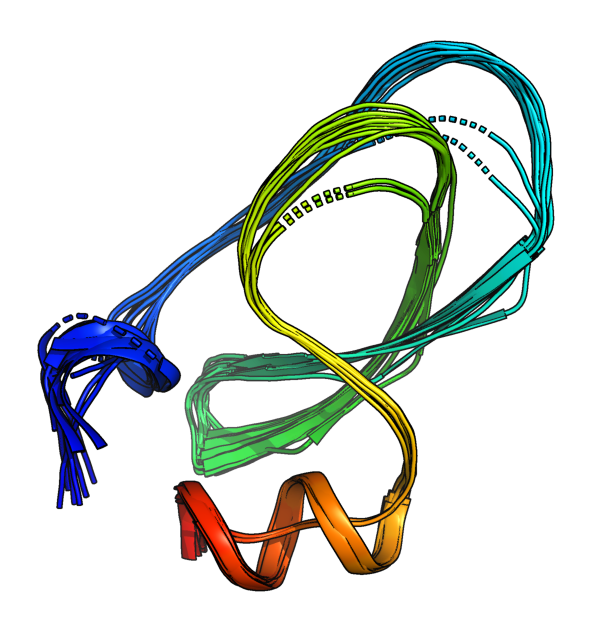
\includegraphics[width=.8\columnwidth]{kunitz_nohelix_cropped}
    \caption{Superposition of the seed structures at the core level. Image obtained with PyMol \citep{pymol2015}.}
    \label{fig:seed}
\end{figure}

\begin{figure}[!tbp]
    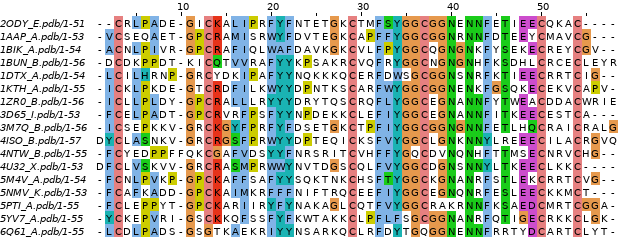
\includegraphics[width=\columnwidth]{msa}
    \caption{Multiples sequence alignment of the seeds. Image obatined with Jalview 2 \citep{jalview2009}}
    \label{fig:ali}
\end{figure}

\begin{figure*}[!t]
    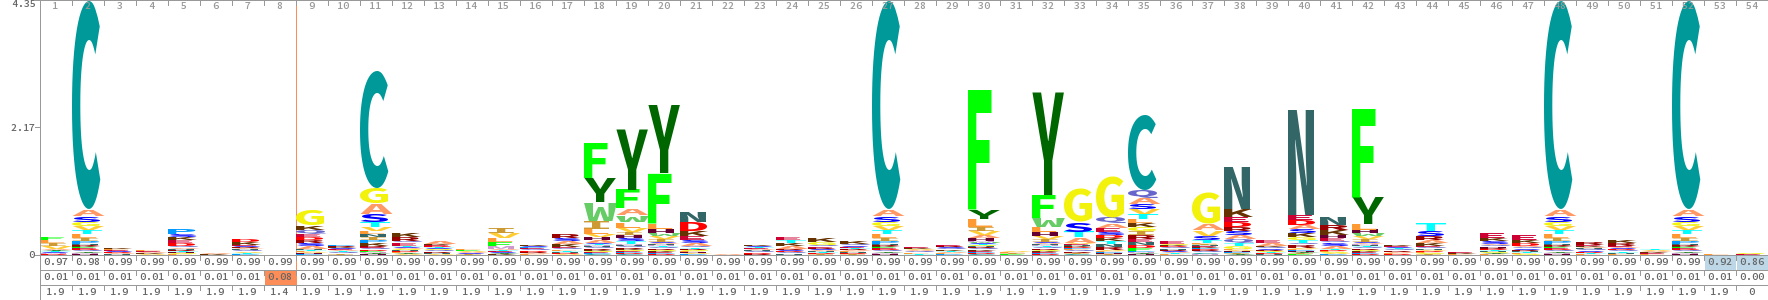
\includegraphics[width=\textwidth]{onlyxray_logo}
    \caption{HMM logo of the BPTI/Kunitz domain. Generated by Skilign \citep{skylign2014}.}
    \label{fig:logo}
\end{figure*}

\subsection{Validation of the profile}
The \texttt{hmmsearch} against the full dataset exhibits a marked class separation between positives and negatives (Figure \ref{fig:whole_plot}).
Consequently, the 5-fold cross validation procedure reported very few mismatches with no difference in classification among the E-values of the best domain and hit.
The average thresholds for the datasets were \num{1.43387082e-9} for the global and \num{2.54107082e-9} for the best domain (Table \ref{tab:01}).
In both instances the false negatives are: Q11101, D3GGZ8, O62247 whereas the only false positive is G3LH89.
A detalied view on the performances on each of the folds is reported in Table \ref{tabS:02}.

\sisetup{round-precision=5}
\begin{table}[!h]
\processtable{Summary of the performance for both datasets. \label{tab:01}} {
\begin{tabular}{@{}cccc@{}}
\toprule Dataset & Avg. E-value & Avg MCC & Avg Accuracy\\
\midrule
Global & \num{1.43387082e-9} & \num{0.994146015207021} & \num{0.9999928855371865}\\
Best domain & \num{2.54107082e-9} & \num{0.994146015207021} & \num{0.9999928855371865}\\
\botrule%
\end{tabular}
}
{}
\end{table}


\begin{figure}[!tbph]
	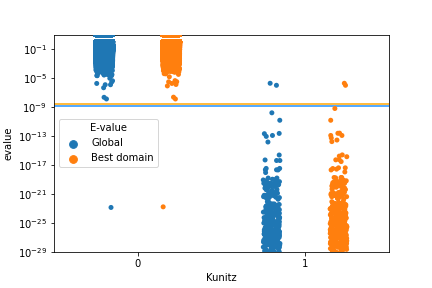
\includegraphics[width=\columnwidth]{whole_plot}
	\caption{Scatterplot of the entire dataset. E-values smaller that $10^{-20}$ are omitted for clarity purposes. The two horizontal lines are the average of the E-value thresholds for both datasets. Image obtained with Seaborn \citep{matplotlib2007}.}
	\label{fig:whole_plot}
\end{figure}
\section{Discussion}
The manual curation of the seed alignment was made possible by the limited amount of proteins that satisfied the initial requirements (i.e. have any structure and a Kunitz domain).
Such approach would not have been possible if there were a more substantial quantity of entries to begin with, at least with this very workflow.
A possible solution to tackle a wider search space for the seeds may be an iterative approach, in which an initial, manually curated, seed is used to identify the most related sequences.
Such procedure can be done iteratively until most of the search space has been scanned, to account for the natural diversity of the sequences that make up the domain.
Nevertheless, the approach described here demonstrated how even a fistful of high-quality structures can be used in building a HMM that is effectively a representative of the domain.
This was possible also because of the nature of the domain in study; indeed, the conservation of very important residues (i.e. the cysteines) necessary to achieve a proper fold plays favorably to our advantage.
The outstanding capabilities of HMMs in domain pattern recognition are well reflected also in our study.
The quality of the seeds made possible to build a model with virtually no noise, which in turn led to a strong class separation in the screening phase.
With these premises, the subsequent cross-validation procedure so trivial that it would have been possible to perform it even by hand.
The basic algorithm involved in the training successfully placed the E-value cutoff threshold in each of the five subsets.
The misclassification of G3LH89 has not really to be taken into account, since it was wrongly labeled to begin with.
The criteria to label as positive only the entries with an associated Kunitz Pfam domain backfired, since many other databases (e.g. Gene3D, SUPFAM, PROSITE) rightfully place it among the other Kunitz domain bearing proteins.
Two false negatives (D3GGZ8 and O62247) are borderline cases.
In fact, even though they are thought to belong to the Kunitz family, their serine-protease inhibition capabilities are disputed, as they are though to be involved in the cuticle formation pathway \citep{pageBiosynthesisEnzymologyCaenorhabditis2006, stepekKunitzDomainProtein2010}.
Finally, Q11101 has no controversial aspects beside its poor annotation.
It would be interesting to see in the future how the improvement annotations, alongside the increased availability of structures will reflect on the performance of this kind of classifiers.
As for now, with the data at hand we can hardly question their efficiency.

\FloatBarrier
\bibliographystyle{natbib}
\bibliography{MyLibrary.bib}

\begin{supplementary}
\section*{Supplementary material}

\begin{table*}[!h]
\processtable{Summary of the seed candidates\label{tabS:01}} {
\begin{tabular}{@{}ccccc@{}}
\toprule Uniprot ID & Representative PDB ID & UniProt Name & Experimental Method & Exclusion reason\\
\midrule
P05067 & 1AAP:A & A4\textunderscore HUMAN & XRC\\
P02760 & 1BIK:A & AMBP\textunderscore HUMAN &XRC \\
Q8WPI2 & 2ODY:E & BOOH2\textunderscore RHIMP & XRC \\
P00974 & 5PTI:A & BPT1\textunderscore BOVIN & XRC \\
P12111 & 1KTH:A & CO6A3\textunderscore HUMAN & XRC \\
A0A1Z0YU59 & 5M4V:A & MAMB1\textunderscore DENAN & XRC \\
O43278 & 4ISO:B & SPIT1\textunderscore HUMAN & XRC \\
O43291 & 4U32:X & SPIT2\textunderscore HUMAN & XRC \\
P10646 & 5NMV:K & TFPI1\textunderscore HUMAN & XRC \\
P48307 & 1ZR0:B & TFPI2\textunderscore HUMAN & XRC \\
Q90WA1 & 3D65:I & VKT1\textunderscore PSETT & XRC \\
P31713 & 3M7Q:B & VKT1\textunderscore STIHL & XRC \\
G9I929 & 4NTW:B & VKTA\textunderscore MICTN & XRC \\
P00989 & 1BUN:B & VKTH2\textunderscore BUNMU & XRC \\
P00980 & 1DTX:A & VKTHA\textunderscore DENAN & XRC \\
P81658 & 5YV7:A & VKTHC\textunderscore DENAN & XRC \\
P0C1X2 & 6Q61:A & VKTS1\textunderscore CONST & XRC \\
Q5ZPJ7 & & VKT\textunderscore NAJAT &  & Only NMR structure available\\
C0HLB2 & & VKT\textunderscore PSEPC &  & Only NMR structure available\\
P68425 & & VKT1A\textunderscore CYRSC & & Only NMR structure available\\
P0DJ46 & & VKT21\textunderscore LYCMC & & Only NMR structure available\\
P25660 & & VKT9\textunderscore BUNFA & & Only NMR structure available\\
P00979 & & VKTH1\textunderscore DENPO & & Only NMR structure available\\
P00981 & & VKTHK\textunderscore DENPO & & Only NMR structure available\\
Q96NZ8 & & WFKN1\textunderscore HUMAN & & Only NMR structure available\\
P12023 & & A4\textunderscore MOUSE & & No structure available \\
P08592 & & A4\textunderscore RAT & & Only fragmented structures \\
Q06481 & & APLP2\textunderscore HUMAN & & No structure available \\
P84875 & & PCPI\textunderscore SABMA & & Only mutant structures \\
Q7TQN3 & & WFKN2\textunderscore MOUSE & & No structure available \\
\botrule%
\end{tabular}
}
{}
\end{table*}

\sisetup{round-precision=5}
\begin{table*}[!h]
\processtable{Detailed performance of the classifier for global E-value and best domain E-value datasets. \label{tabS:02}} {
\begin{tabular}{@{}lccccccccc@{}}
\toprule Sample               & True negatives & True positives & False positives & False negatives & Selected E-value threshold   & Train Accuracy               & Train MCC                & Test Accuracy            & Test MCC						\\
\midrule
Fold 1 - Global               & 112379         & 69 		    & 0 			  & 0 			    & \num{1.7782794100389228e-09} & \num{0.9999933301911123} & \num{0.9944937520518929} & \num{1.0}                & \num{1.0}\\  
Fold 2 - Global               & 112379         & 67 		    & 0 			  & 2 			    & \num{5.6234132519034906e-11} & \num{0.9999955534706273} & \num{0.9963347717220772} & \num{0.999982213842966} & \num{0.9853919077406604}\\
Fold 3 - Global               & 112378         & 68 		    & 0 			  & 0 			    & \num{1.7782794100389228e-09} & \num{0.9999933302059411} & \num{0.9945138663196862} & \num{1.0} & \num{1.0}\\
Fold 4 - Global               & 112379 	       & 67 		    & 0 			  & 1 			    & \num{1.7782794100389228e-09} & \num{0.9999955534706273} & \num{0.9963481403436356} & \num{0.999991106921483} & \num{0.9926154089702117}\\
Fold 5 - Global               & 112379 	       & 68 		    & 1 			  & 0 			    & \num{1.7782794100389228e-09} & \num{0.9999955534706273} & \num{0.9963414641492768} & \num{0.999991106921483} & \num{0.9927227593242328}\\

Fold 1 - Best domain               & 112379         & 69 		    & 0 			  & 0 			    & \num{1.7782794100389228e-09} & \num{0.9999933301911123} & \num{0.9944937520518929} & \num{1.0}                & \num{1.0}\\  
Fold 2 - Best domain               & 112379         & 67 		    & 0 			  & 2 			    & \num{5.6234132519034906e-11} & \num{0.9999955534706273} & \num{0.9963347717220772} & \num{0.999982213842966} & \num{0.9853919077406604}\\
Fold 3 - Best domain               & 112378         & 68 		    & 0 			  & 0 			    & \num{1.7782794100389228e-09} & \num{0.9999933302059411} & \num{0.9945138663196862} & \num{1.0} & \num{1.0}\\
Fold 4 - Best domain               & 112379 	       & 67 		    & 0 			  & 1 			    & \num{1.7782794100389228e-09} & \num{0.9999955534706273} & \num{0.9963481403436356} & \num{0.999991106921483} & \num{0.9926154089702117}\\
Fold 5 - Best domain               & 112379 	       & 68 		    & 1 			  & 0 			    & \num{1.7782794100389228e-09} & \num{0.9999955534706273} & \num{0.9963414641492768} & \num{0.999991106921483} & \num{0.9927227593242328}\\

\botrule%
\end{tabular}
}
{}
\end{table*}
\end{supplementary}
\end{document}
